\begin{opin}{\guscolor}{Gustavo}

\subsubsection{Introducción a la neurodidáctica}

Parece una evidencia científica que sin emoción no hay aprendizaje. Es necesario despertar en los adolescentes el interés por las matemáticas en particular y por el conocimiento en general. Y para ello podemos hacer uso de técnicas que permitan emocionar a los alumnos sobre lo que están haciendo y de esta manera conseguir que, seguramente de manera inconsciente para ellos, aprendan los contenidos básicos necesarios para su desarrollo personal.


Hay gente que equipara los términos neurodidáctica y neuroeducación, ambos asociados a la neurociencia. En nuestra clase lo vamos a diferenciar en función de:

\begin{itemize}
\item Neuroeducación: Manera en la que el cerebro aprende
\item Neurodidáctica: Manara en la que el docente lleva a la práctica la neuroeducación
\end{itemize}

\subsubsection{Neuroeducación por otra escuela}

Se puede acceder al video en el siguiente enlace:

\href{https://www.youtube.com/watch?v=QiRqCKUiRDc\&feature=youtu.be}{https://www.youtube.com/watch?v=QiRqCKUiRDc\&feature=youtu.be}
\paragraph{Partes del cerebro. Aprendizaje =  DIVERSION * K}
Las cosas que yo pienso \textmd{se ejecutan} mediante la parte del cerebro prefrontal, que sería la parte de la cabeza que usan los futbolistas para rematar un balón. Se denomina función ejecutiva y se encarga de:
\begin{itemize}
\item La concentración
\item El control de impulsos
\item La memoria a corto plazo
\end{itemize}
La amígdala es la parte del cerebro que se encarga de la emoción y es “la gasolina” de la función ejecutiva.


\begin{minipage}[hbtp]{1.0\linewidth}
\centering
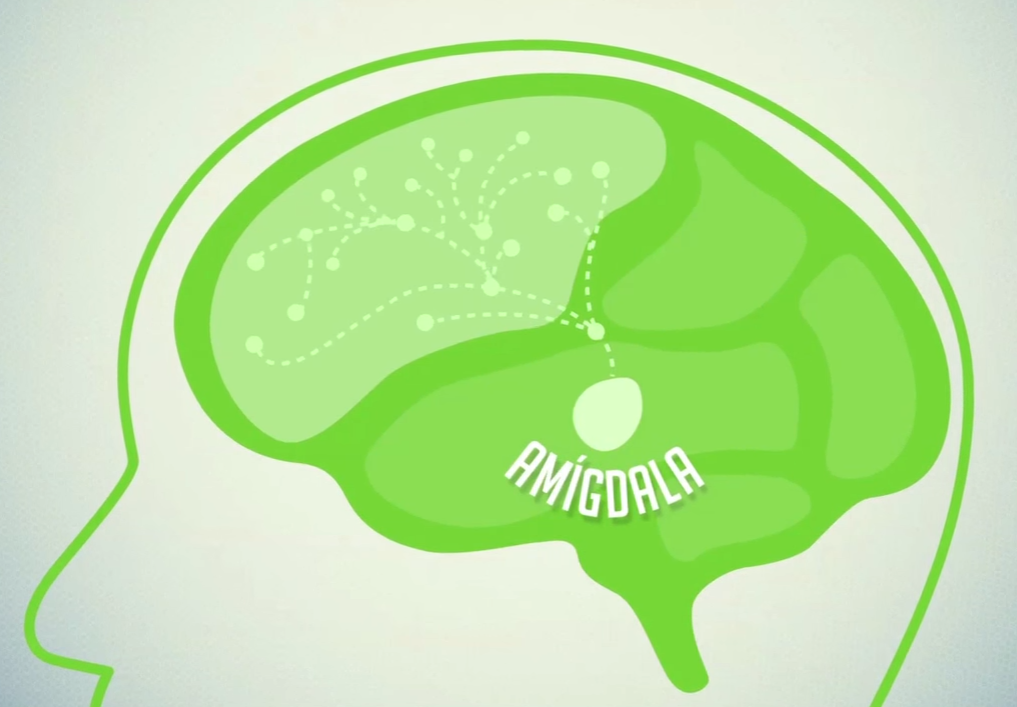
\includegraphics[scale=0.2]{img/cerebrogus.png}
\captionof{figure}{Esquema de la posición de la amígdala en el cerebro humano.}
\end{minipage}

Por simplificar mucho hasta el momento, la parte racional está en el prefrontal y la parte emocional está en la amígdala.


Con esto se explicaría que si estás emocionado con algo, tengas una mejor concentración y por tanto un mejor aprendizaje. En realidad, el cerebro tiene muchas partes y para que el proceso de aprendizaje sea total se deberían emplear todas las regiones y funciones del cerebro.


Como dijo \textbf{Helena Lopez Casares en la conferencia que dio el 20 de septiembre en el Campus Vicálvaro} sobre inteligencias múltiples, hay estudios que demuestran que personas con problemas en la parte del cerebro que controla las emociones son incapaces de tomar una decisión, con lo cual se demuestra la importancia de todas las partes del cerebro deben estar activas y conectadas.

\paragraph{Educación bulímica. Matemáticas, Historia y Filosofía}
Me ha gustado mucho la afirmación que hace Javier Blumenfeld: “Tenemos una especie de educación bulímica: yo te meto contenidos y tú me los vomitas en el examen”. Esto es lo que yo llamo metodología tradicional de la enseñanza.


En este caso sí haría diferenciación por asignaturas y lo aplicaría a mi experiencia personal. En el caso de las matemáticas, aparte de que siempre me han gustado más, he sido capaz de aprenderlas y es muy difícil que se me olviden. O si hay algo que no tengo claro, con un simple repaso sería capaz de recordarlo. Estas matemáticas las he aprendido bajo un contexto de educación bulímica y aun así he sido capaz de aprenderlas. Sin embargo, en asignaturas como historia, filosofía, u otras asignaturas que la manera de aprobar consistía en la memorizar y repetir lo memorizado en el examen, no he recordado nunca nada de adulto.


Sin embargo, es curioso como a día de hoy sí me siento atraído por la historia y por los pensamientos filosóficos. Bajo mi punto de vista es que este cambio se debe a que he alcanzado unos conocimientos y una madurez que me permiten disfrutar de ello. No tenía ningún sentido estudiarlo con la edad que tenía. No disfrutaba de ello. Hace poco hice un tour que te lleva por el Madrid de los Austrias con guía y lo disfruté muchísimo, cosa que era impensable cuando era un niño. Este sería un claro ejemplo de que cuando algo te gusta lo aprendes mejor. Aunque en este caso concreto, tengo la opinión de que es muy difícil motivar a unos alumnos que no han vivido los suficientes años como para entender y disfrutar de la historia y de los filósofos.


\paragraph{Buscando culpables}
En el punto anterior he hecho una exposición desde mi propia experiencia personal. Sin embargo, tengo compañeros y amigos que sí que han sido capaces de aprender más cosas de historia que yo en etapas tempranas de la vida.


¿Cuál será el motivo por el que yo NO he aprendido historia y otras personas que conozco sí? 
¿Será que el colegio en el que ellos estudiaban, fueron capaces de emocionarles mejor en Historia? 
¿O será que yo nunca he puesto interés? 
Tenemos que tener cuidado también con aquellos alumnos que se aprovechen de esto para decir que no han aprendido lo suficiente alegando que el sistema educativo no era el adecuado o que las metodologías de aprendizaje no eran las adecuadas. Hay que hacer analizar todas las situaciones de manera individual para poder discernir aquellos alumnos que realmente han sido sometidos a altos niveles de estrés que han limitado su capacidad de aprendizaje de aquellos alumnos que simplemente no ponían interés.


\paragraph{Entendido el problema. Y ahora …?}
Una vez hecho el diagnóstico de la situación y entendido que como docentes tenemos que motivar para conseguir emocionar al alumnado y de esta manera conseguir que el aprendizaje sea más efectivo, lo que hay que ver ahora es cómo llevar a cabo ese cambio.


Pero antes de empezar a analizar las diferentes alternativas que se plantean como los trabajos por proyectos, aprendizaje basado en problemas, etc me gustaría lanzar una pregunta abierta sin ánimo de criticar estas iniciativas de cambio y es la siguiente, ¿Qué pasaría si con el cambio ocurre que hay alumnos que no se sienten motivados por estas nuevas metodologías? Podríamos volver al problema del cual partimos y volveríamos a tener alumnos desmotivados. Según esto, lo ideal sería una enseñanza personalizada en el individuo y no en el grupo. Pero por otro lado, vivimos en sociedad, somos seres sociales y una enseñanza individual podría dar lugar a perder otro tipo de conocimientos sociales muy importantes. La conclusión es que podamos combinar una educación en la que cada uno aprenda a su velocidad pero en sociedad.

\paragraph{Mens sana in corpore sano}
Me ha interesado mucho también el estudio que asocia deporte con aprendizaje.


Tener alumnos sentados durante tanto tiempo en el aula es antinatural. Después de hacer un ejercicio, sobre todo aeróbica el cerebro funciona mejor.


La irisina se genera al hacer deporte y baja de los músculos al cerebro y favorece la plasticidad neural, que es la base del aprendizaje.


En este caso, las imágenes que aparecen en las transparencias de clase son muy significativas. Se ha evolucionado en muchos aspectos de la vida y sin embargo parece que las aulas permanecen “incambiadas” desde hace muchos años.
\end{opin}


\begin{opin}{\victorcolor}{Víctor}



\subsubsection{Charla de neurodidáctica}

Aunque no es propiamente de la asignatura, es gracias a la profesora, Raquel Garrido,  que fui a la jornada complementaria sobre \textbf{Neuroeducación}.
%
En este charla, además de tratar conceptos como la \textit{amígdala}, comentada por Gustavo anteriormente, tratamos del \index{TDAH}\textbf{TDAH} (Trastorno Déficit de Atención e Hiperactividad). 
%
El ponente hacía una reflexión muy interesante: \textit{Se medica para que el chaval con un trastorno neurológico se adaptara al método. 
%
Tal vez el problema no está en el trastorno neurológico sino en la metodología empleada.} para concluir un poco después: \textit{Con la manera de dar clase se puede contrarrestar totalmente el TDAH de un alumno.}
%
Esta reflexión me hizo también ser consciente de la importancia que tiene mi labor. 
%
De hecho, nos contaba un caso de su clínica en el que un chaval tendría que ser medicado si le tocaba el profesor de Matemáticas A pero se podría evitar la medicación si su profesor de Matemáticas era B, porque así había sido otros años. ¡Qué responsabilidad!

En esta charla se dió una clave muy importante para tratar con alumnos con TDAH:\textit{
Hay una diferencia entre no aprender y aprender pero no ser capaz de retomar ese conocimiento aprendido. 
%
Una persona con TDAH puede aprender, pero su frontal no es capaz de retomar la información.}

Por último, resumo otra idea que me resultó esclarecedora:
%
Atender es un acto involuntario, la concentración es consciente. 
%
No podemos pedir que nos presten atención (porque es involuntario). Necesitamos captar su atención. 
%
Por otro lado,
la concentración es la selección voluntaria de uno de los focos a los que atendemos. 
%
Sí podemos pedirles que se concentren en lo que estamos haciendo, ya que eso sí depende del alumnado.




\end{opin}

\begin{opin}{\pedrocolor}{Pedro}


Durante esta sesión se ha introducido el término “neurociencia” con sus dos vertientes: neuroeducación y neurodidáctica.  Hasta la fecha, eran conceptos totalmente desconocidos para mí, pese a su presencia desde hace casi 25 años.

El término neuroeducación trata de aprovechar el conocimiento sobre cómo aprende el cerebro, mientras que la neurodidáctica está orientada a acercar el conocimiento de la neurociencia a la aplicación metodológica dentro del aula.

Para poder entender un poco como funciona el cerebro en un proceso de aprendizaje, podemos diferenciar tres partes:

\begin{itemize}

\item \textbf{\textit{Cerebro Límbico o Cerebro Emocional:}} No hay conciencia sobre su actuación, y por lo tanto no se ejerce ningún control sobre él. Tiene capacidad de producir “emociones”. Esto nos lleva a concluir que las emociones son incontrolables, lo que somos capaces de controlar son las conductas asociadas a las emociones.    

\item \textbf{\textit{Cerebro Cognitivo o Cerebro Pensante:}} Reconoce la señal enviada por el Límbico y actúa de forma inconsciente. 

\item \textbf{\textit{Cerebro Ejecutivo o Lóbulo Frontal:}} Es la parte del cerebro que me permite autocontrolar mis emociones actuando de forma consciente, convirtiéndose en el director de orquesta del cerebro.  La función ejecutiva tiene tres partes, la primera la “Concentración”, la segunda parte “El Control de Impulsos” y la tercera parte es “La Memoria a Corto Plazo”. Las amígdalas generan neurotransmisores que hacen que esta función ejecutiva en el Lóbulo frontal se encuentre activa (gasolina del Cerebro ejecutivo). Por eso cuando algo me gusta o emociona soy capaz de estar concentrado, por lo tanto hay que hacer que los alumnos segreguen dopamina (neurotransmisor). 

\end{itemize}

El Lóbulo Frontal es la parte del cerebro que falla a los alumnos no TDAH:

\begin{itemize}

\item Carecen de su capacidad de inhibición que les permitan no ser impulsivos. 

\item Sin capacidad para autorregular las emociones. 

\item Dificultad para establecer metas de forma consciente.  

\item Baja capacidad de perseverancia y voluntad propia. 

\item Poca capacidad en el control interno del tiempo, autoevaluación, automonitorización y  concentración. 

\end{itemize} 

 

Una de las partes que más me ha llamado la atención es el concepto de “neuronas espejo”. El principal motor del aprendizaje es la imitación y esto se produce en este tipo de neuronas, reflejando en nuestro interior lo que vemos fuera, tanto a nivel motor, como a nivel de motivación, creatividad etc. Esto pone de manifiesto como el aprendizaje cooperativo es más potente que cualquier clase magistral.

Me gustaría hacer referencia a Javier Blumenfled y José Ramón Gamo. La asistencia a su Jornada sobre Neuroeducación y TDAH me ha permitido tomar conciencia de los diferentes modos de operación del cerebro humano, según la edad o el tipo de dificultades asociadas a cada alumno. Para concluir me quedo con una frase de cada uno de ellos:

\begin{itemize}

\item La educación bulímica no genera un aprendizaje significativo. (Javier Blumenfled) 

\item El maestro que se compromete con un alumno le salva la vida.  (José Ramón Gamo) 
\end{itemize}
 

Mis aportaciones audiovisuales sobre este tema:

Francisco Mora Teruel: \url{https://www.youtube.com/watch?v=8E3Y-t6j0GE}   

Conferencia José Ramón Gamo: \url{https://www.youtube.com/watch?v=fNzjKGRIJt0&t=4562s}

\end{opin}

\begin{opin}{\virgicolor}{Virginia}

En este tema aparecieron términos nuevos para mí que no había oído hasta ahora como son la \textbf{neuroeducación}\index{neuroeducación} y la \textbf{neurodidáctica}\index{neurodidáctica}, ambas relacionadas entre sí. La neuroeducación estudia cómo aprende el cerebro y la neurodidáctica como comenta el especialista en Neuropsicología Infantil José Ramón Gamo es el método de enseñanza que se basa en la capacidad de aprendizaje del cerebro en el que se distingue la parte cognitiva, la emocional y la ejecutiva. Me parece muy interesante esta disciplina ya que si conocemos bien cómo funciona el cerebro del ser humano podemos facilitar el aprendizaje del mismo.

Quiero destacar el vídeo que nos puso Raquel, Neuroeducación: por otra escuela en el que hablan David Bueno, Ana Forés y Javier Blumenfeld: \url{https://www.youtube.com/watch?v=QiRqCKUiRDc&feature=youtu.be}


Me parece realmente interesante porque destaca distintos puntos que son vitales para la compresión de estos nuevos conceptos introducidos:

\begin{itemize}

\item Partes del cerebro: destaca en la parte frontal del cerebro la función ejecutiva. Esta actúa como el motor del cerebro el cuál necesita tener bien los sistemas que se encargan de la emoción que es otra parte del cerebro que se llama amígdala (gasolina de la función ejecutiva) (ver figura \ref{viramigdala}). La amígdala potencia que la función ejecutiva esté activa de forma que como dice Javier Blumenfeld “cuando estoy emocionado soy capaz de aprender mejor”. 

 

\item Aprendizaje según maduración del cerebro. Me pareció muy interesante ya que los contenidos de cada curso deberían tener en cuenta la maduración del cerebro del alumno ya que no tiene sentido enseñar algo que no son capaces de aprender porque puede ser contraproducente ya que se sentirían incapaces, se estaría posiblemente creando una indefensión aprendida al adelantar objetivos que aún no son capaces de asumir.   

 

\item Estrés. En este punto me siento especialmente reflejada ya que cuando me he sentido agobiada por la carga de trabajo mi cerebro ha actuado peor y he necesitado parar y relajarme para poder continuar trabajando mejor. Es decir, se debe evitar que los alumnos se sientan estresados para conseguir un adecuado aprendizaje. No hay que cargarles de deberes sin entender realmente los conceptos que realmente deben aprender porque si no se conseguirá que asocien el aprendizaje como algo estresante y negativo en lugar de como algo positivo y muy importante para su futuro. 

\item Neuronas espejos. En este punto tratan la importancia del trabajo colaborativo y aprender unos de otros ya que las neuronas espejo reflejan aquello que vemos fuera. Javier destaca que “el aprendizaje colaborativo es mucho más potente porque se enciende nuestras neuronas espejos” y Ana Forés recalca que “el cerebro trabaja mejor colaborativamente que no competitivamente”. 

 
\item Ejercicio físico. Según dice David Bueno el alumno tiene que ser el sujeto activo tanto mentalmente como activamente: “la educación física libera una sustancia que favorece la plasticidad neural que es la base del aprendizaje”. Estoy totalmente de acuerdo en el que el deporte ayuda al aprendizaje porque entre otras cosas te libera la mente y te desestresa, lo que deja a tu cerebro libre para adquirir nuevos conocimientos. En mi caso, yo me siento mucho más productiva después de realizar algún deporte además de más contenta, y desde luego el aprendizaje se ve favorecido si tu estado anímico es mejor. 

\end{itemize}


En definitiva y para concluir lo visto en este vídeo creo que es verdaderamente importante crear un nuevo sistema de \textbf{aprendizaje que sea permanente y que nos guste y emocione}. En una entrevista que le hacen a Javier Blumenfield en cuatro explica: “Si me gusta, mis motores de aprendizaje entienden más y eso permite que el aprendizaje llegue a una parte más profunda de mi cerebro”. Aquí dejó el link a esa entrevista:

\url{http://www.cuatro.com/cintoraapiedecalle/temporada-1/t01xp02-malditos-deberes/Javier-Blumenfeld-pediatra-habla-educacion_2_2150955229.html}


%%%%%%%%%%%%%%% TAMAÑO IMGS Y CAPTION



Después de ver el vídeo Neuroeducación: por otra escuela, seguimos tratando en clase la función ejecutiva. En este punto entendí el comportamiento de los adolescentes ya que lo último que se desarrolla en la maduración del cerebro es la función ejecutiva. Como esta incluye las destrezas para organizar y planificar una tarea a realizar inhibiendo las distracciones, entendí el por qué los adolescentes dicen lo primero que se les pasa por la cabeza sin pensar si está bien o mal ya que lo hacen sin una planificación y una organización y sin inhibirse al no tener su función ejecutiva desarrollada. Por tanto, el correcto desarrollo de esta función es muy importante para saber cómo comportarse en cada momento y que actitudes tomar de forma organizada y sensata.

\begin{minipage}[hbtp]{1.0\linewidth}
\centering
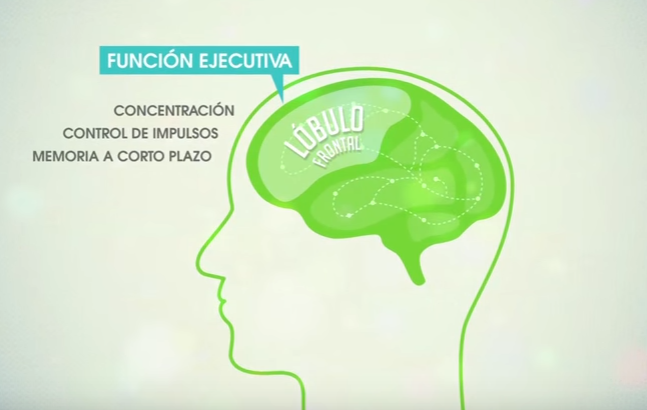
\includegraphics[width=0.4\linewidth]{img/viryi1.png}
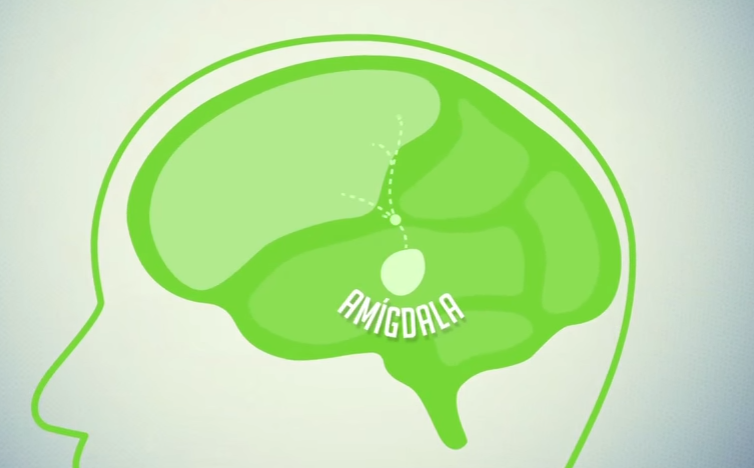
\includegraphics[width=0.408\linewidth]{img/viryi2.png}
\captionof{figure}{Función ejecutiva (motor del cerebro) Amígdala (gasolina)}
\label{viramigdala}
\end{minipage}


En este punto se trató el experimento de Walter Mischel, Marshmallow experiment. A pesar de que ya lo conocía me resultó muy interesante la conexión con la función ejecutiva de la que no había oído hablar de forma técnica. Curiosamente, hace poco fui a ver una obra de teatro “El test” en la que el tema principal es la siguiente pregunta: \textit{¿qué prefieres 100.000 euros ahora o 1 millón de euros dentro de 10 años”?} Digamos que sería la equivalencia en un adulto al experimento con chuches del niño. En esta obra, hay una psicóloga que compara ambos test en el que la conclusión al final es la misma: que el niño o adulto que ha sabido esperar, en el futuro consiguen mejores trabajos y son más felices.

%\begin{minipage}{1.0\linewidth}
%\centering
%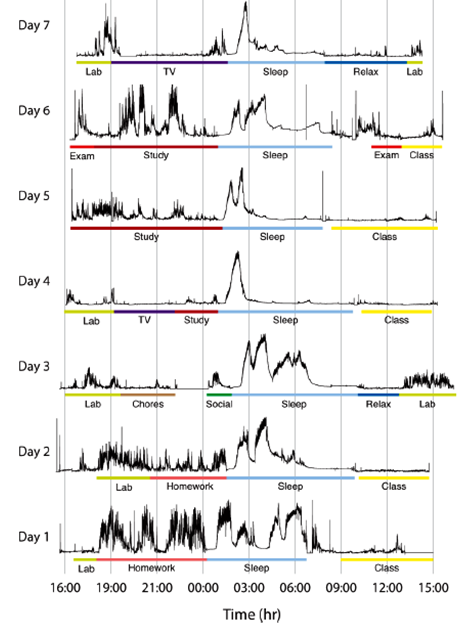
\includegraphics[scale=0.6]{img/viryi3.png}
%\captionof{figure}{ Registro de actividad electrodérmica de un universitario durante 24h en su casa y en clase en actividades cotidianas (Poh, Swenson y Picard, 2010)}
%\label{estudiomolon}
%\end{minipage}



%%%%%%%%%%%%%%%% COMPROBAR NO SOLAPAN TEXTOS

%\textcolor{red}{Comprobar solapamiento de textos.}

\vspace{2cm}
\end{leftbar}
\vspace{-2cm}
\begin{figure}[hbtp]
\begin{leftbar}{\virgicolor}
%\vspace{1cm}
\centering
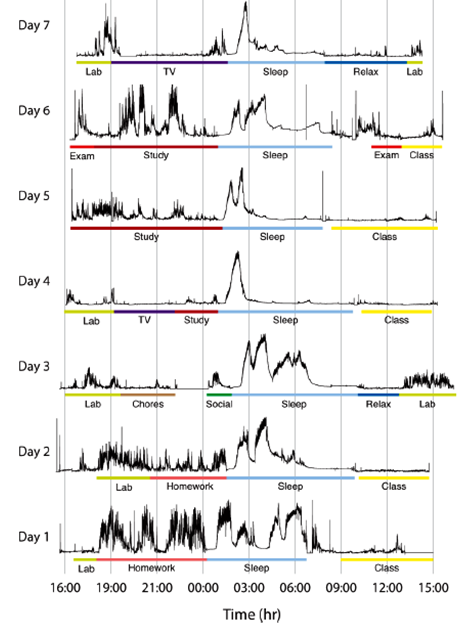
\includegraphics{img/viryi3.png}
\caption{Registro de actividad electrodérmica de un universitario durante 24h en su casa y en clase en actividades cotidianas (Poh, Swenson y Picard, 2010)}
\label{estudiomolon}
%\vspace{2cm}
\end{leftbar}
\end{figure}
%\vspace{-2cm}
\begin{leftbar}{\virgicolor}


De los documentos complementarios que nos cuelga Raquel en aula virtual me pareció muy interesante el artículo sobre \textit{“Actividad cerebral del alumno durante la tradicional clase magistral”}.
En el estudio se muestra que los mayores picos de actividad se obtienen en la realización de los deberes, en el trabajo de laboratorio, durante los exámenes y en periodos de estudio debido a la mayor exigencia cognitiva de dichas tareas. Por el contrario, la amplitud y la frecuencia de las ondas registradas decaían mucho cuando el alumno estaba escuchando las clases magistrales de su profesor obteniéndose un nivel de actividad fisiológica similar al que se producía cuando se encontraba viendo la televisión e incluso al que se da en alguna de las fases características de relajación durante el sueño (ver Figura \ref{estudiomolon}). Viendo estos resultados está claro que hay que actuar cambiando la metodología tradicional, porque si el cerebro no se activa y no se emociona no va a aprender. Así, la aplicación de la neurodidáctica creo que es vital en la educación para conseguir que lo que se enseñe se aprenda.




Por motivos de trabajo y muy a mí pesar no pude asistir a la charla que dieron Javier Blumenfeld y José Ramón Gamo. 
%
Afortunadamente he podido ver algunas charlas de ellos en Internet. 
%
Ya hice anteriormente algún comentario sobre una entrevista que vi de Javier y ahora toca el turno de hablar de una charla que dio José Ramón Gago en la universidad Rey Juan Carlo (\url{https://www.youtube.com/watch?v=ZBhUfVVktYw}). 
%
Me hizo gracia cuando cuenta la historia del sabio que dice que enseñó a hablar a su perro y nadie le creía, pero entonce el sabio responde “He dicho que he enseñado a hablar a mi perro lo que no quiere decir que mi perro haya aprendido a hablar”. 
%
Lo que quiere decir todo esto es que todo lo que está en nuestras manos como futuros profesores es enseñar. 
%
Por tanto, hay que buscar métodos adecuados de enseñanza para que lo que enseñemos sea aprendido por los alumnos. 
%
José Ramón Gamo dice en su charla “hay que partir del conocimiento de la neurociencia para seleccionar cuales son las metodologías que acompañan mejor la enseñanza natural de un cerebro”. 
%
Explica también que no aprendemos solos porque el cerebro es un órgano social que necesita trabajar de forma colaborativa. 
%
Para finalizar el comentario de este vídeo y que además sirve de base como introducción al siguiente apartado (Emociones y aprendizaje) José Ramón explica que los mecanismos básicos para el aprendizaje son la motivación, la atención y las memorias que se activan gracias a la emoción. 
%
En definitiva, \textbf{el cerebro aprende emocionándose. }

\end{opin}
